\newpage
\section{Auswertung}
    \subsection{Statische Methode}
        Bei der statischen Methode wird jeweils an zwei Stellen eines jeden Metallstabes die Temperatur als Funktion der Zeit gemessen und über den zeitlichen
        Temperaturverlauf wird an den beiden Messstellen die Wärmeleitfähigkeit der vier Metallstäbe bestimmt.

        \subsubsection{Temperaturverläufe der fernen Thermoelemente}
        Im folgenden befindet sich eine Grafik für alle fernen Thermoelemente. Dabei misst das Thermoelement $T1 \si{second}$ an dem dicken Messingstück und $T4 \si{second}$ am dünnen. $T5 \si{second}$ und $T8 \si{second}$ sind
        jeweils am Aluminium und Edelstahl befestigt.

        \begin{figure}
               \centering
               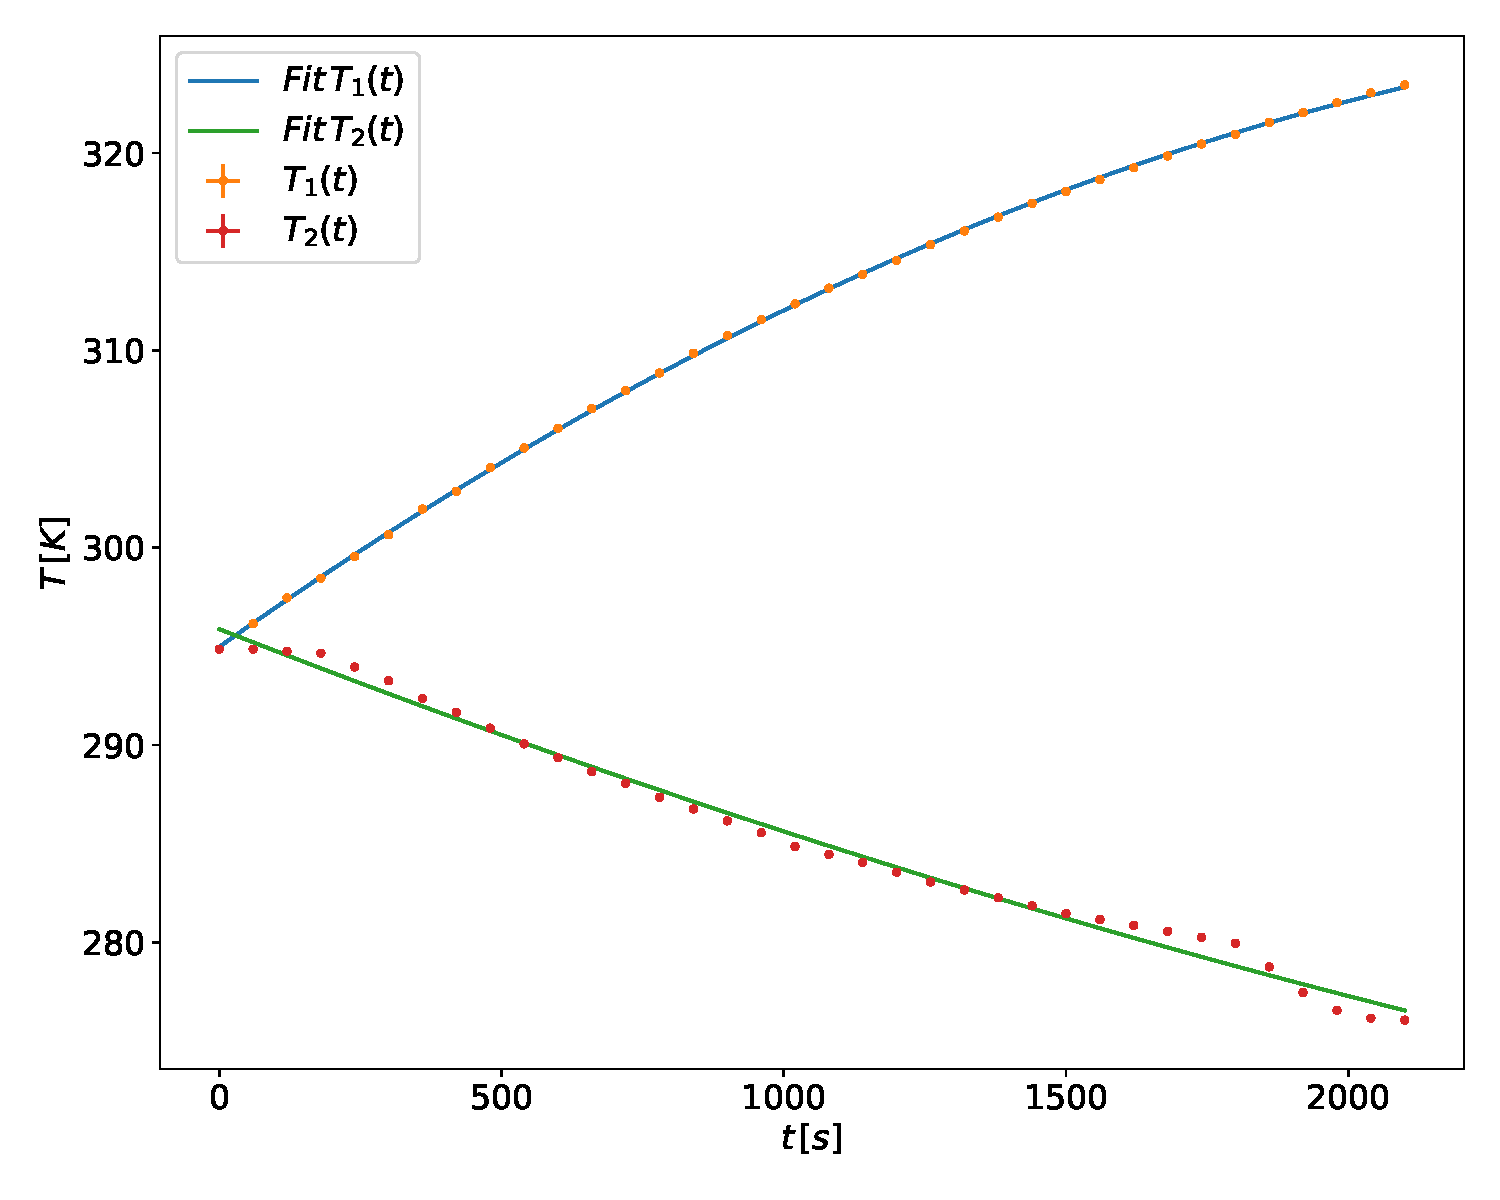
\includegraphics[width=\textwidth]{Daten/grafic.pdf}
               \caption{Temperaturverläufe der fernen Thermoelemente $T1$, $T4$, $T5$, $T8$}
               \label{fig:static_far}
        \end{figure}

        Es fällt auf, dass $T1$ und $T4$ ungefähr von $t = 0 \si{\second}$ bis $t = 100 \si{\second}$ gleichstark steigen, jedoch steigt die Temperatur von $T5$ deutlich steiler und von $T8$ deutlich 
        flacher als die gemessene Temperatur der anderen Thermoelemente.
        Zudem ist bei allen Thermoelementen, außer bei $T8$, ab $t = 600 \si{\second}$ ein starker Knick zu beobachten. Außerdem steigt $T8$ nicht sofort, sowie die anderen Kurven direkt, sondern verzögert. 
        Es ist außerdem auffällig das alle Kurven nach dem Abflachen nahezu parallel verlaufen.


        An den Graphen lässt sich jeweils die Temperaturen bei 700s ablesen.
        \begin{align}
         T1(700 \si{\second}) &=  318.06 \si{\kelvin} \\ 
         T4(700 \si{\second}) &=  316.42 \si{\kelvin} \\
         T5(700 \si{\second}) &=  320.66 \si{\kelvin} \\
         T8(700 \si{\second}) &=  318.06 \si{\kelvin} 
        \end{align}

        Aus der Grafik lässt sich erkennen, dass die Temperatur von T5 bei 700s am größten ist. Daraus lässt sich schlussfolgern, dass die Wärmeleitfähigfkeit von Aluminium im Vergleich zu Edelstahl und Messing am besten ist.

        \subsubsection{Wärmestrom}
        Mit der Gleichung (\ref{eqn:waermemenge}) lässt sich nach einer Umstellung zu $\frac{\symup{d}Q}{\symup{d}t} $ der Wärmstrom als differenz $\frac{\Delta Q}{\Delta t} $ berechnen.
        
        \begin{table}
        \centering
            \begin{tabular}{
                S[table-format=3.0]
                S[table-format=1.4]
                S[table-format=1.4]   
                S[table-format=1.4]
                S[table-format=1.4]
            }
            \toprule
            {$t \mathbin{/} \si{\second} $} & {$\kappa_\text{Messing(Dick)} \si[per-mode=fraction]{\watt\per\meter\per\kelvin} $}
            & {$\kappa_\text{Messing(Dünn)} \si[per-mode=fraction]{\watt\per\meter\per\kelvin} $}
            & {$\kappa_\text{Aluminium} \si[per-mode=fraction]{\watt\per\meter\per\kelvin} $}
            & {$\kappa_\text{Edelstahl} \si[per-mode=fraction]{\watt\per\meter\per\kelvin} $} \\
            \midrule
            0   & 0.038 & -0.052 & 0.011 & -0.018 \\
            100 & 0.917 & -0.569 & 0.700 & -0.346 \\
            200 & 0.634 & -0.420 & 0.474 & -0.300 \\
            300 & 0.566 & -0.387 & 0.435 & -0.272 \\
            400 & 0.552 & -0.377 & 0.431 & -0.259 \\
            \bottomrule
            \end{tabular}
        \caption{Messdaten}
        \label{tab:5_Mess}
        \end{table}
        
        \subsection{Diagramme der Temperaturdifferenzen}

    \begin{figure}
        \begin{subfigure}{0.48\textwidth}
               \centering
               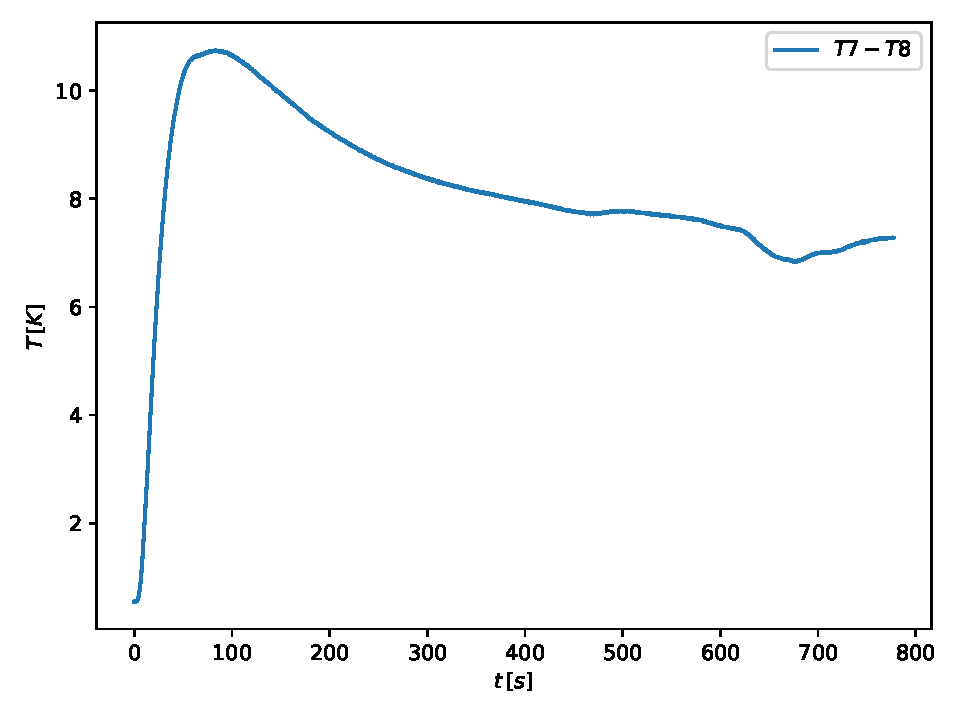
\includegraphics[height=5.5cm]{Daten/grafic1.pdf}
               \caption{Temperaturverlauf von $T7-T8$}
               \label{fig:static_T7-T8}
        \end{subfigure}
    \hfill
        \begin{subfigure}{0.48\textwidth}
               \centering
               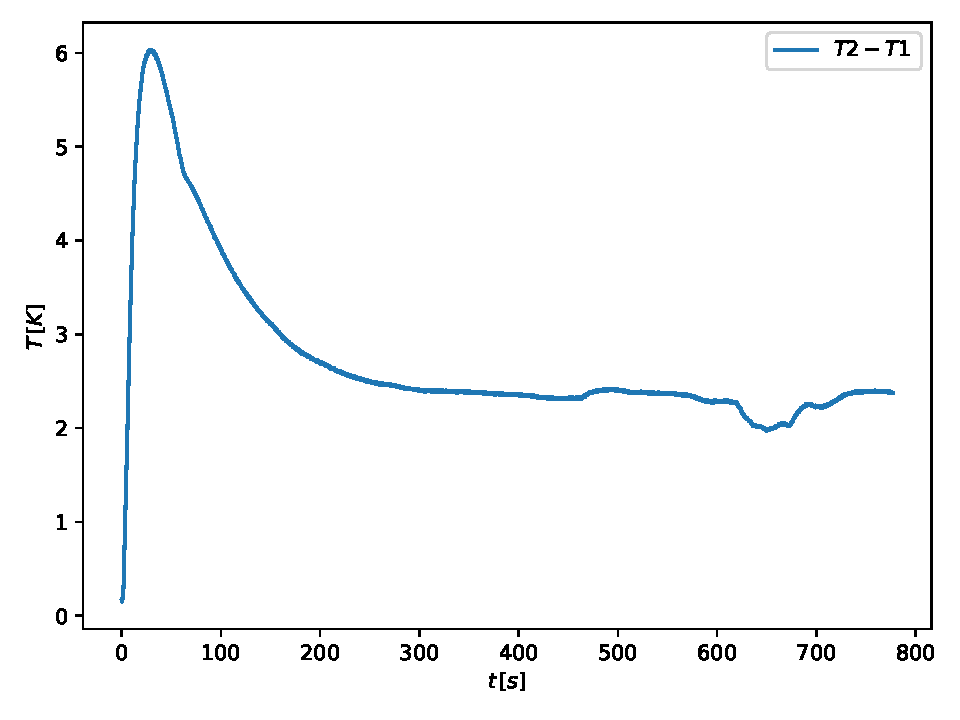
\includegraphics[height=5.5cm]{Daten/grafic2.pdf}
               \caption{Temperaturverlauf von $T2-T1$}
               \label{fig:static_T2-T1}
        \end{subfigure}
    \end{figure}

    Es fällt auf das beide Graphen mit einer ungefähr gleichen Steigung steigen. Zudem flachen beide Graphen bei großem t relativ stark ab und haben beide eine "Kuhle" ab ungefähr t=630s.
    Außerdem haben beide einen Hochpunkt bei ungefähr t=50s. 

Jedoch fällt der Graph von $T2-T1$ deutlich stärker als $T7-T8$. Das globale Maximum von $T7-T8$ liegt ebenfalls höher, als $T2-T1$. Wenn man allerdings genau hinschaut, bei den beiden Globalen Maxima,
    dann sieht man, dass das Messing vor dem Edelstahl sein Maximum annimmt. 

    Der geringe Abfall von $T7-T8$ und der hohe Graph, sowie das höhere Maxima deutet darauf hin, dass die Wärmeleitfähigkeit von Edelstahl signifikant schlechter ist als von Messing. Dies lässt sich auch in den
    errechneten Wärmeleitfähigkeiten sehen.

    \subsection{Dynamische Methode mit einer 80s Periode}

    Im folgenden sind die beiden Temperaturverläufe für den breiten Messingstab (T1 und T2), bei einem Umschalten von 'HEAT' auf 'COOL' alle 40s, graphisch dargestellt.
    \begin{figure}
        \begin{subfigure}{0.48\textwidth}
               \centering
               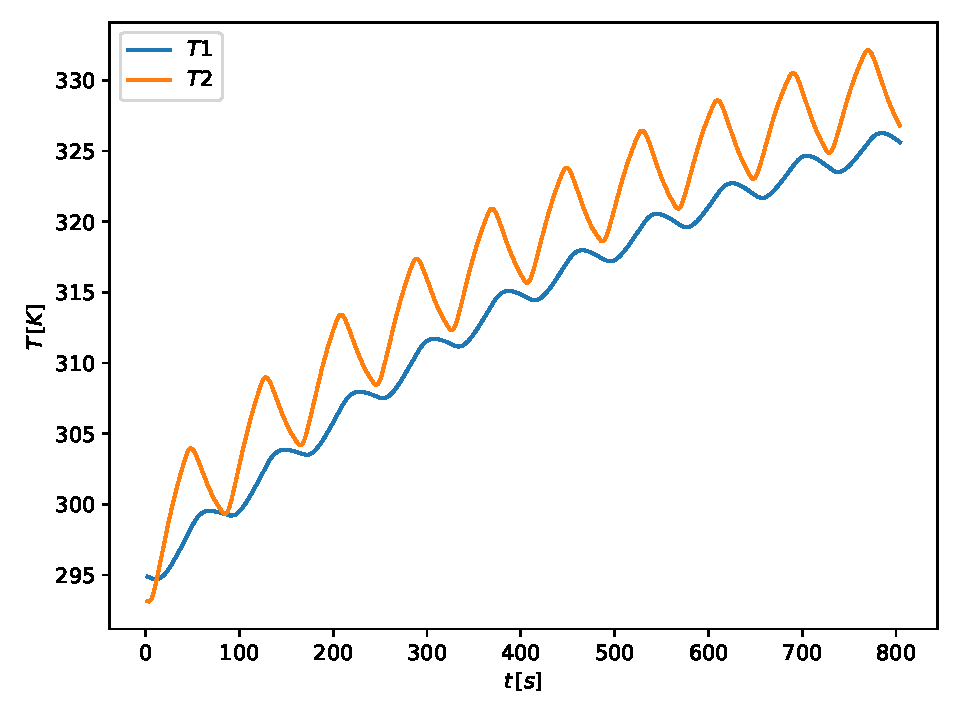
\includegraphics[height=5.5cm]{Daten/grafic3.pdf}
               \caption{Temperaturverlauf von $T1$ und $T2$}
               \label{fig:dyn_T1}
        \end{subfigure}
    \hfill
        \begin{subfigure}{0.48\textwidth}
               \centering
               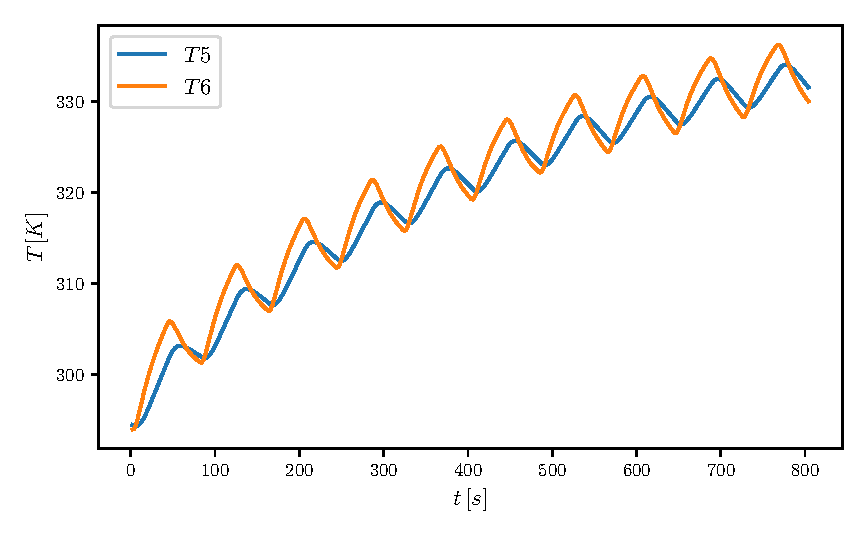
\includegraphics[height=5.5cm]{Daten/grafic5.pdf}
               \caption{Temperaturverlauf von $T5$ und $T6$}
               \label{fig:dyn_T5}
        \end{subfigure}
    \end{figure}
    
    Aus der Grafik lassen sich die Größen der Amplituden A1 und A2, sowie Phasendifferenz $\Delta t$ für Messing und Aluminium ermitteln. Dabei werden von vielen Perioden die Amplituden bestimmt und dann gemittlet. (Da jedoch die Daten in Digitaler Form vor lagen wurden diese rechnerisch bestimmt):
    \begin{table}
        \centering
            \begin{tabular}{
                S[table-format=1.1]
                S[table-format=1.1]
                S[table-format=1.3]   
                S[table-format=1.1]
                S[table-format=1.2]
                S[table-format=1.4]
            }
            \toprule
            {$A1_\text{Messing} \si{\kelvin} $}
            & {$A2_\text{Messing} \si{\kelvin} $}
            & {$\Delta t_\text{Messing} \si{\second} $}
            & {$A5_\text{Aluminium} \si{\kelvin} $}
            & {$A6_\text{Aluminium} \si{\kelvin} $}
            & {$\Delta t_\text{Aluminium} \si{\second} $}\\
            \midrule
            5.2 & 4.3   & 0.981 & 4.8 & 4.22 & 0.518 \\
            \bottomrule
            \end{tabular}
        \caption{Errechnete Daten aus den Graphen}
        \label{tab:MesAlu}
    \end{table}

    Mithilfe dieser Zahlenwerte lässt sich die Wärmeleitfähigkeit $\kappa$ berechnen für das Aluminium und Messing bestimmen. Jedoch weichen die errechneten Zahlen stark von den Literaturwerten ab, sodass wir davon ausgehen,
    dass etwas bei der Berechnung falsch gelaufen ist. Der Fehler ließ sich leider nicht in der gegebenen Zeit finden.

    \begin{table}
        \centering
            \begin{tabular}{
                S[table-format=4.2]
                S[table-format=5.2]
            }
            \toprule
            {$\kappa_\text{Messing} \si[per-mode=fraction]{\watt\per\meter\per\kelvin} $}
            & {$\kappa_\text{Aluminium} \si[per-mode=fraction]{\watt\per\meter\per\kelvin} $}\\
            \midrule
            7142.73 & 16358.29 \\
            \bottomrule
            \end{tabular}
        \caption{Wärmeleitfähigkeit von Aluminium und Messing}
        \label{tab:MesAlu}
    \end{table}


    \subsection{Dynamische Methode mit einer 200s Periode}
    

    Die selbe Auswertung die bei Aluminium und Messing erfolgte, erfolgt jetzt ebenfalls bei Edelstahl, bei welchem ein Umschalten von 'HEAT' auf 'COOL' alle 100s erfolgt. Jedoch wurde diesmal von vielen Perioden die Amplitude bestimmt und jeweils die Wärmeleitfähigfkeit $\kappa$ ausgerechnet und nicht nur leidglich mit der gemittleten Amplitude.
    
    \begin{figure}
               \centering
               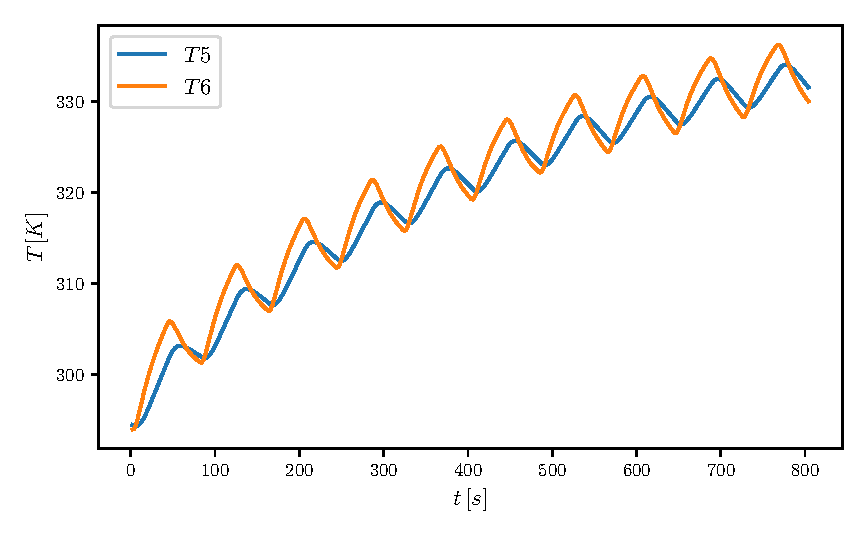
\includegraphics[width=\textwidth]{Daten/grafic5.pdf}
               \caption{Temperaturverläufe der Thermoelemente $T7$ und $T8$}
               \label{fig:dyn_edel}
        \end{figure}

    \begin{table}
        \centering
            \begin{tabular}{
                S[table-format=2.0]
                S[table-format=2.0]
                S[table-format=1.2]   
                S[table-format=4.3]
            }
            \toprule
            {$A7_\text{Edelstahl} \si{\kelvin} $}
            & {$A8_\text{Edelstahl} \si{\kelvin} $}
            & {$\Delta t_\text{Edelstahl} \si{\second} $}
            & {$\kappa_\text{Edelstahl} \si[per-mode=fraction]{\watt\per\meter\per\kelvin} $}\\
            \midrule
            49 & 1   & 24.6 & 289.326 \\
            49 & 15   & 24.56 & 951.203 \\
            50 & 1   & 24.86 & 287.832 \\
            51 & 74   & 18.23 & -3024.950 \\
            \bottomrule
            \end{tabular}
        \caption{Errechnete Daten aus den Graphen}
        \label{tab:MesAlu}
    \end{table}